\documentclass[12pt, preprint]{aastex}

% words
\newcommand{\project}[1]{\textsl{#1}}
\newcommand{\documentname}{\textsl{Article}}
\usepackage{color}
\bibliographystyle{apj}

\usepackage{hyperref}
\newcommand{\niceurl}[1]{\href{#1}{\textsl{#1}}}


% To-do:
%  - Author names: initials or full names?
%  - do we get the same result with the official WISE coadds (vs unWISE)?
%  - which legacysurvey.org URL to list?
%  -> viewer in L,B ?
%  - Galactic L,B grid lines?
%  - ensure that Figure 1 galactic L,B are labelled correctly!  Is the LMC in the right place?

\newcommand{\viewerurl}{\niceurl{http://legacysurvey.org/viewer}}

\begin{document}

\title{The Milky Way has an X-shaped bulge} 
\author{%
M.~Ness\altaffilmark{1,2},
D.~A.~Lang\altaffilmark{3,4}
}
%
\shortauthors{Ness, Lang}
\altaffiltext{1}{%
  Max-Planck-Institut f\"ur Astronomie,
  K\"onigstuhl 17, D-69117 Heidelberg, Germany
}
\altaffiltext{2}{%
  To whom correspondence should be addressed:
  ness@mpia-hd.mpg.de
}
\altaffiltext{3}{%
  Department of Astronomy \& Astrophysics and Dunlap Institute,
  University of Toronto,
  50 Saint George Street, Toronto, ON, M5S 3H4, Canada
}
\altaffiltext{4}{%
  Department of Physics \& Astronomy,
  University of Waterloo,
  200 University Avenue West, Waterloo, ON, N2L 3G1, Canada
}

\begin{abstract}%
The Milky Way bulge has a boxy/peanut morphology and an X-shape structure. This X-shape has been revealed by the `split in the red clump' from 
star counts along the line of sight toward the bulge, measured from photometric surveys. An alternative scenario proposes that the bulge is not X-shaped and that the apparent split in the red clump is instead due to different stellar populations, in an old classical spheroidal bulge. We present a WISE image of the Milky Way bulge, produced by downsampling the publicly available ``unWISE'' coadds.  The WISE image of the Milky Way bulge shows that the X-shaped nature of the Milky Way bulge is self-evident and irrefutable. This data used to create this image that we present is publicly available and can be readily accessed by the community for further analysis of the nature of the X-shaped bulge of the Milky Way. 
\end{abstract}
%The X-shaped property the Milky Way's bulge has been recently questioned. An alternative scenario to the X-shaped morphology, to explain the split in the red clump stars in the inner Galaxy has been proposed that the bulge is not X-shaped and the apparent

\keywords{%
}

\section{Introduction}\label{sec:Intro}

% A metallicity dependence of this
%split in the red clump has also been determined by spectroscopic surveys. N-body models of boxy/peanut bulges formed via disk instabilities demonstrate that the X-shape is a consequence of the orbit families of stars of which it is comprised. 
%
The split in the red clump stars in the Galactic bulge was first detected from photometric surveys \citep{McWilliam2010, Nataf2010}. This split was later determined to be a property of the more metal rich stars in the bulge, with [Fe/H] $>$ --0.5 \citep{Ness2012, Uttenthaler2012}; although according to \citet{Nataf2014} this metallicity dependence may be subject to biases. Using photometric data from the VVV survey, \citet{Wegg2013} measured the three dimensional density of red clump stars in the bulge and determined the distribution to be characteristic of a strong boxy/peanut bulge within a barred galaxy. This boxy nature itself was first revealed in the COBE image \citep{Dwek1995}. \citet{Portail2015a} have used this density map to show that the Milky Way's boxy/peanut bulge has an off-centered X structure. Furthermore, using constraints from kinematic data, \citet{Portail2015b}  determine that the fraction of stars in orbits that contribute to the X-shape is 40 - 45\% of the mass of the bulge. This X-shaped morphology seen in the Milky Way is typical of spiral galaxies that are barred and has been observed in the unsharp masked images of other galaxies \citep[e.g.][]{Bureau2006}. Such an X-shape which underlies the boxy/peanut morphology is seen to form in N-body simulations of bulges formed via disk instabilities \citep[e.g.][]{Athanassoula2005, Debattista2006, Inma2006}. \citet{Portail2015b} have shown the different orbit possibilities beyond the x$_{1}$v$_{1}$ orbit families \citep[e.g.][]{P1991} that can support this structure.



\citet{Lee2015} have questioned the existence of the X-shaped morphology of the bulge, instead proposing the split in the red clump stars to be a consequence of different stellar populations in a classical bulge that are helium enriched. In response, \citet{Gonzalez2015} has recently provided a detailed analysis of the observational properties of the bulge and analysis that reinforces the link between the double or split red clump and the X-shape. We present, for the first time, the WISE image of the Milky Way \citep{Lang2014a} which clearly demonstrates the Milky Way bulge is irrefutably morphologically, X-shaped. This follows expectations from the observational evidence,  from dynamical models of boxy/peanut bulges like the Milky Way, and from observations of other barred galaxies that reveal such an X-shaped morphology is not uncommon \citep{L2014}. 



\section{The WISE image of the Milky Way bulge}

\textcolor{blue}{\textbf{For the following sections in blue text: Is all of this right - have we said enough?} }

The Wide-Field Infrared Survey Explorer (WISE, \citet{W2010}) is a full sky photometric survey using four bands in the mid-infrared at 3.4 $\micron$, 4.6 $\micron$, 12 $\micron$ and 22 $\micron$ (W1--W4).
The original WISE data release was based on a co-adding approach that is optimal for detecting isolated point sources but which effectively blurs the images. \citet{Lang2014b} implemented an alternative co-adding methodology that does not degrade the resolution of the imaging.  These ``unWISE'' coadds have been publicly released\footnote{available at \niceurl{http://unwise.me}}.


Figure \ref{fig:xbulge} presents the WISE image from \citet{Lang2014a} \footnote{available in interactive ra,dec coordinates at \viewerurl} of the bulge region of the Milky Way, $(l,b)$ $<$ (180, 50), resampled to galactic coordinates.  This image shows WISE bands W1 and W2. This presents the overall Milky Way structures in exquisite detail.
No additional unsharp masking or equivalent techniques have been used to enhance these data. The bulge in the central region of this Figure shows a clear X-shaped morphology. Note that the arms of the X-shape are asymmetrical around the minor axis and appear larger at left than at right. This is a real projection effect and reflects that the bulge is oriented at about 27$^\circ$ degrees with respect to the line of sight \citep{Wegg2013}, with the nearest side at positive longitudes.

%Clear features like the small and large magellanic clouds are visible at $(l,b)$ $\approx$ $()$ and the in-plane dust 

\begin{figure}[h!]
\centering
        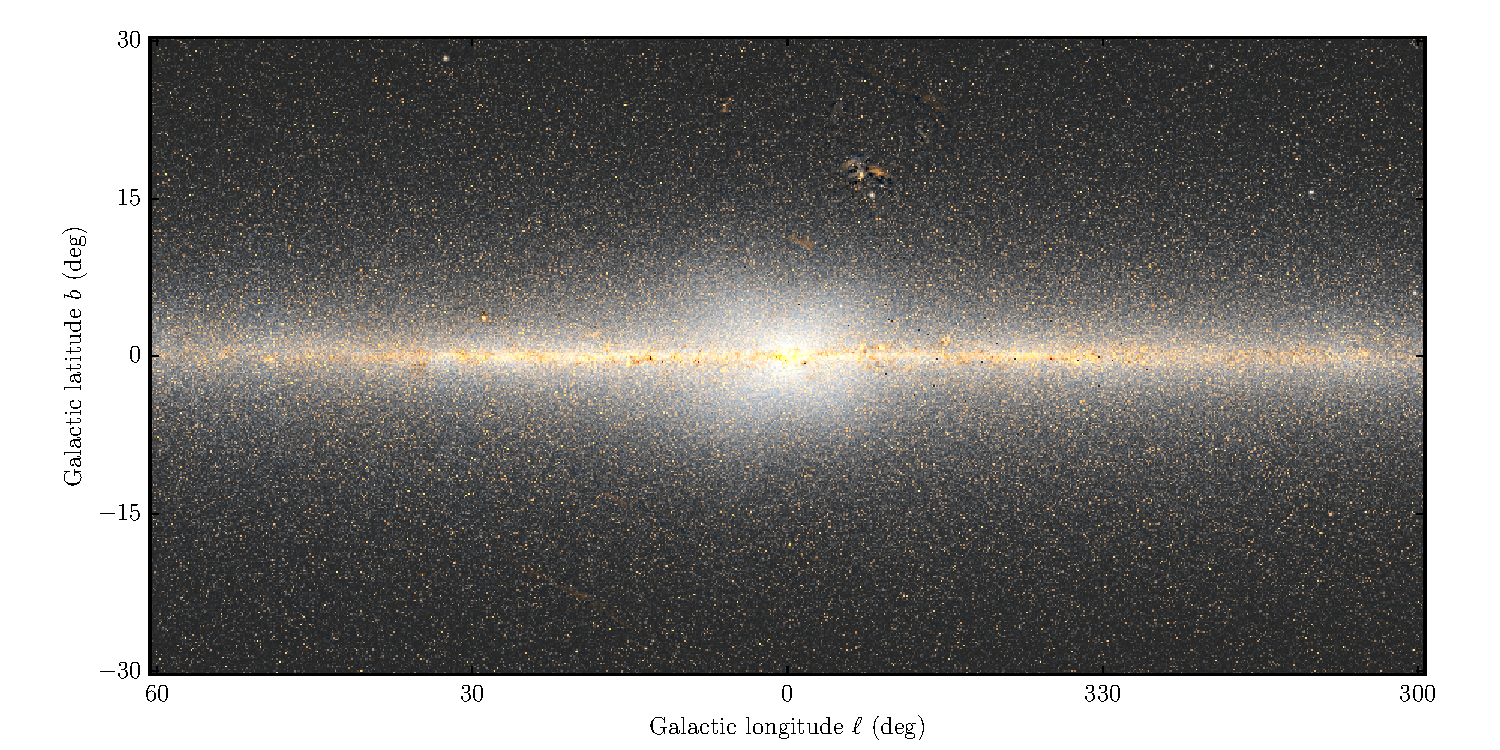
\includegraphics[width=\textwidth]{xbulge-00}
\caption{WISE image for W1 and W2 in Galactic coordinates.  An arcsinh
  stretch is used to allow the full dynamic range to be shown.}
% and put link to webpage where this is: \viewerurl}
\label{fig:xbulge}
\end{figure}

\section{The WISE image of the bulge: contrast enhanced}

\textcolor{blue}{Figure \ref{fig:filt} presents a contrast enhanced and zoomed in version of Figure \ref{fig:xbulge}. This better reveals the X-shape light profile of the bulge and its extent across $(l,b)$ in the WISE image. This Figure was produced with a median subtraction across each row. The arms in the image extend to longitudes of $l$ $\approx$ XX and latitudes of $|b|$ $\lesssim$ XX; (although note again the arms on the near side are larger than those of the far side due to projection). This extent on the sky corresponds to a length of XX kpc for each arm  , for a distance of the bulge of 8kpc from the Sun. }

\begin{figure}[h!]
\centering
        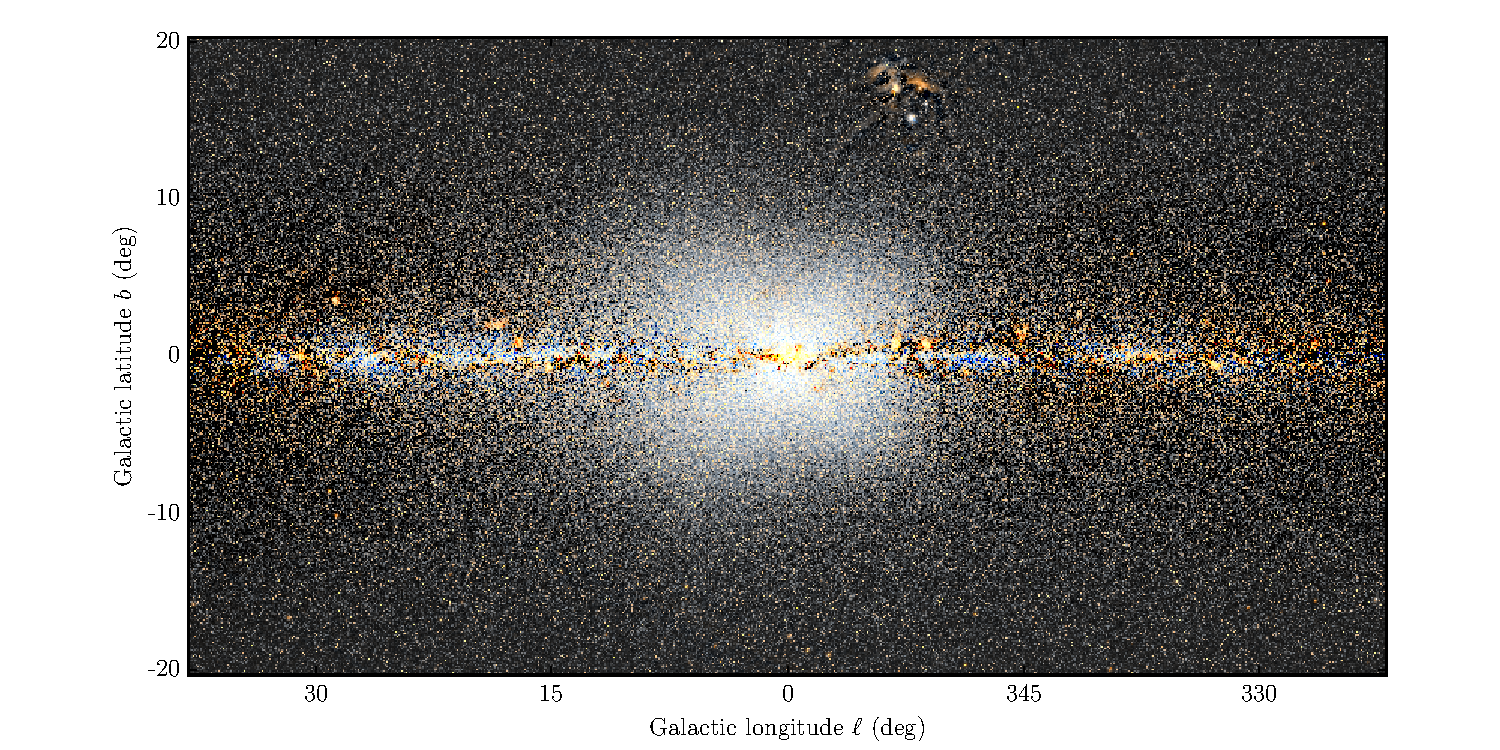
\includegraphics[width=\textwidth]{xbulge-01}
\caption{Same as Figure 1 but zoomed in and with the median of each row of the image subtracted.}
\label{fig:filt}
\end{figure}

\begin{figure}
\centering
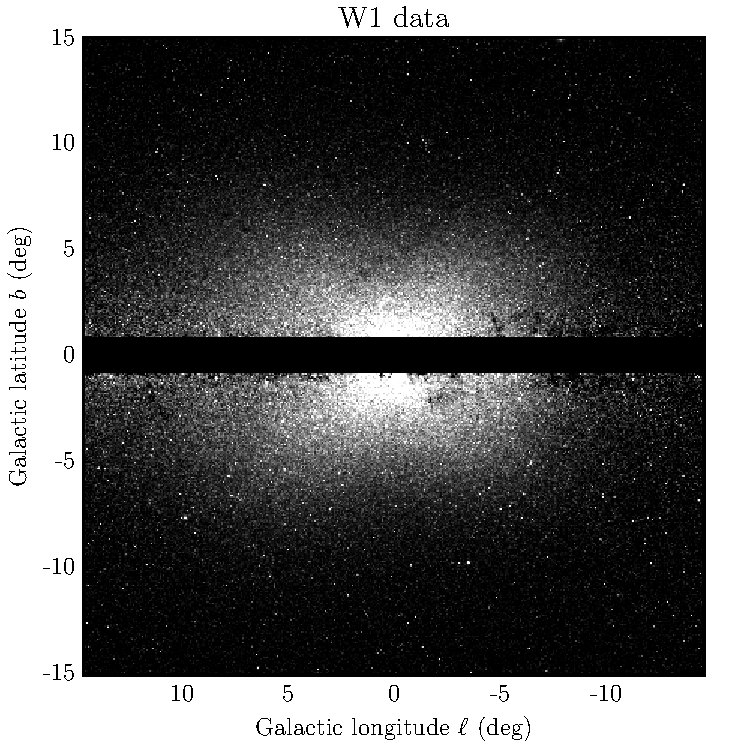
\includegraphics[width=0.3\textwidth]{xbulge-04}
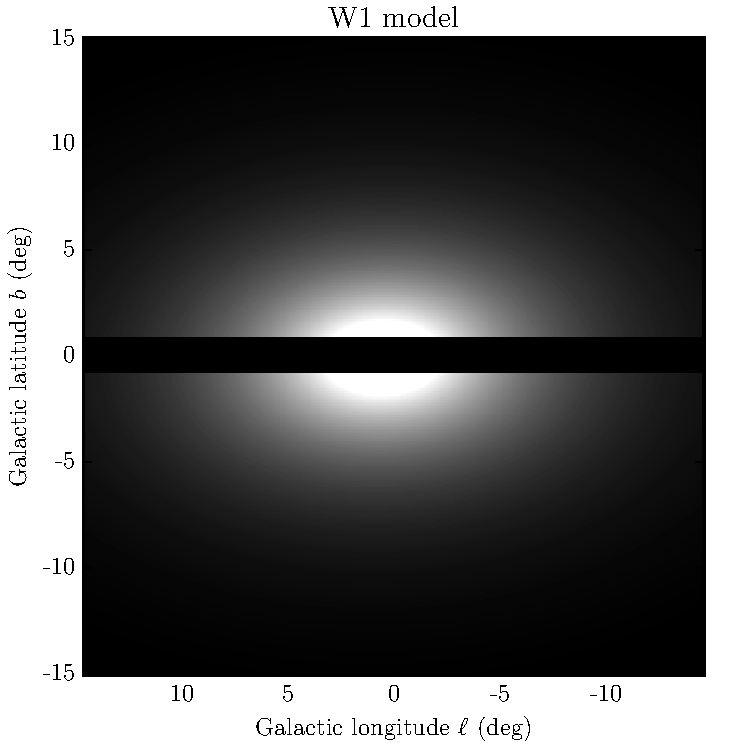
\includegraphics[width=0.3\textwidth]{xbulge-08}
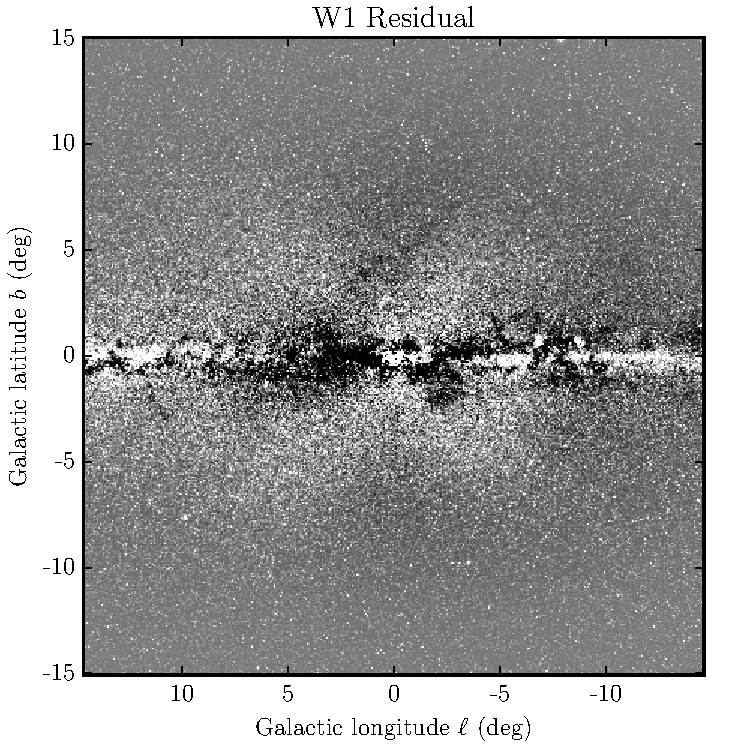
\includegraphics[width=0.3\textwidth]{xbulge-09}
\\
\rule{0.3\textwidth}{0pt}
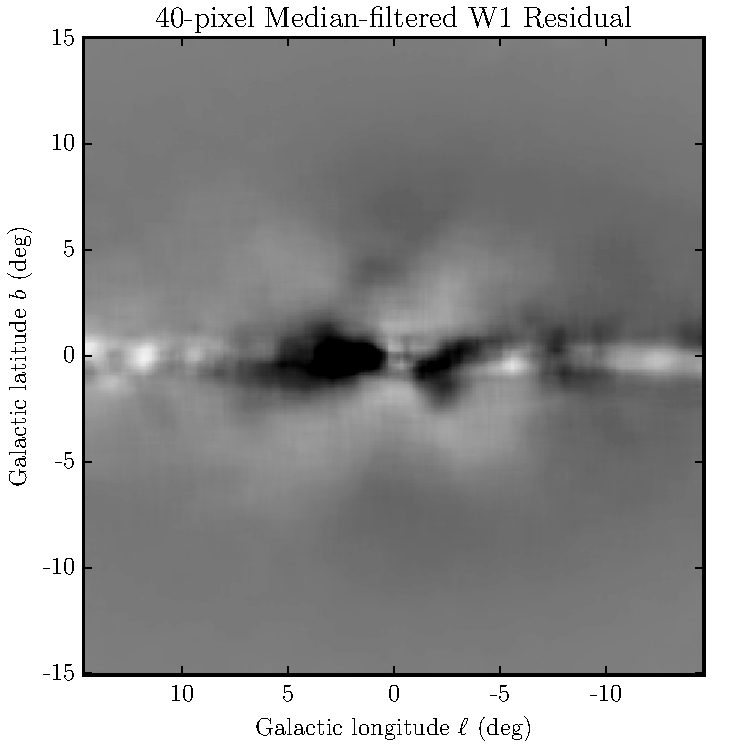
\includegraphics[width=0.3\textwidth]{xbulge-10}
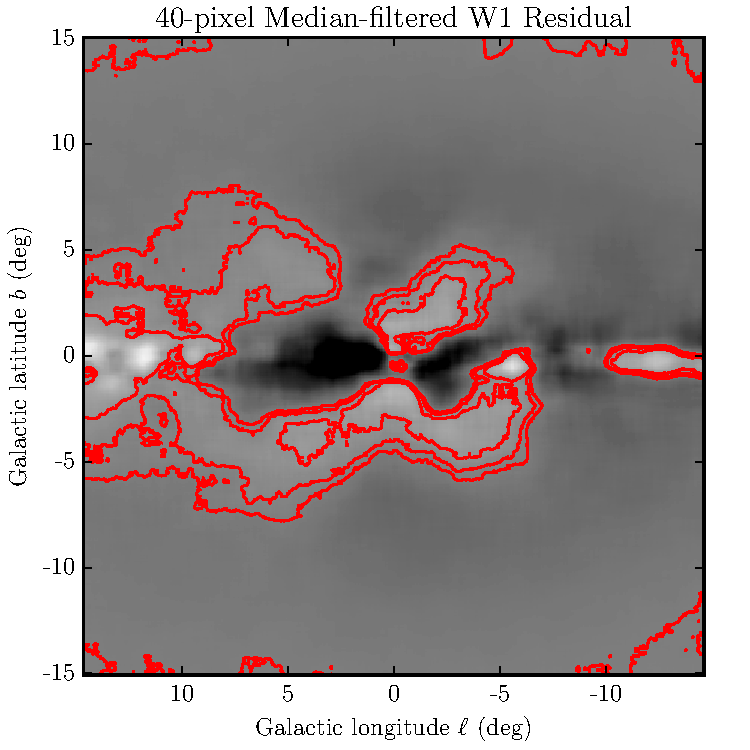
\includegraphics[width=0.3\textwidth]{xbulge-11}
\caption{WISE W1 image fit by a simple exponential disk model, masking
  out the core of the galactic plane.  In the residuals, the X
  structure becomes more apparent, and is evident in the contour plot.}
\label{fig:modfit}
\end{figure}


\begin{figure}
\centering
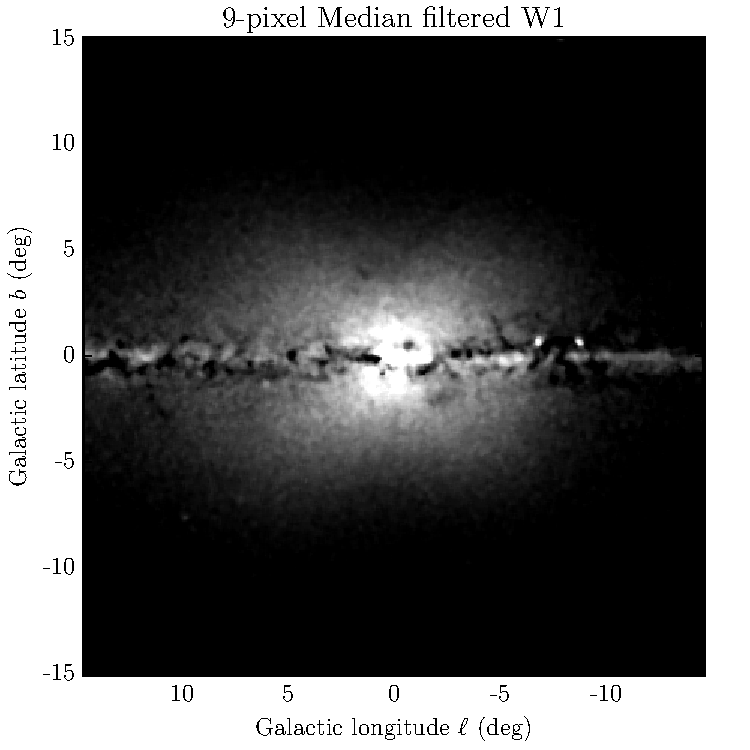
\includegraphics[width=0.3\textwidth]{xbulge-05}
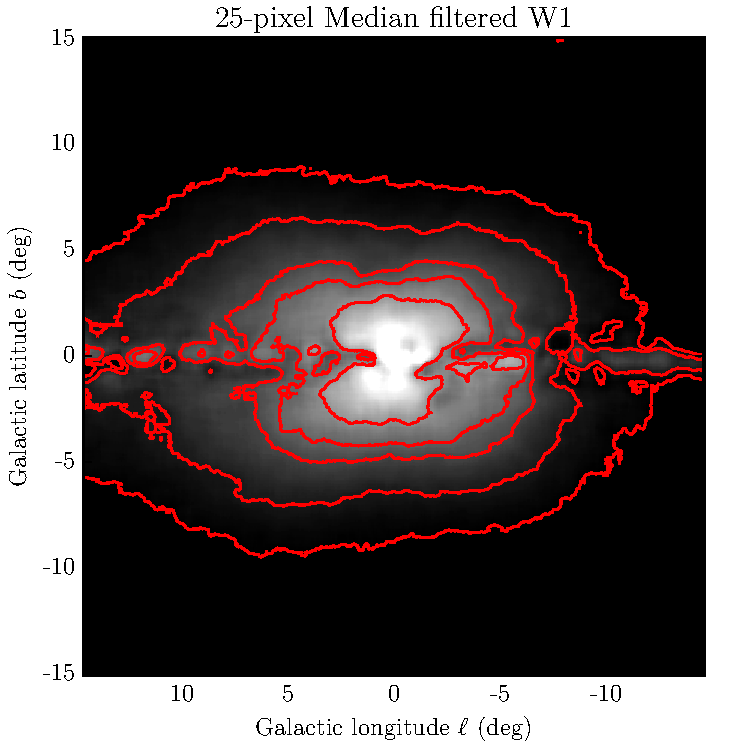
\includegraphics[width=0.3\textwidth]{xbulge-07}
\caption{
}
\label{fig:contours}
\end{figure}


\section{Conclusion}

What to say here?\\
- working on W3 and W4 which will detail bulge further?\\
- this image can be used to directly compare to external galaxies? \\
- shows the bulge has an X-shape; detected years ago now just obvious in looking at a picture of it. \\



\bibliography{Xbulge_bib.bib}

\end{document}

%\section{Alternative Scenario} 
%
%Summarise the alternative scenario \\
%
%\section{WISE image} 
%
%Put in the main wise image and explain how obtained - reference DL unwise me paper \\
%
%section{enhanced contrast image} 
%
%Put in the enhanced contrast image that Dustin sent 
%
%COBE (Dwek et al. 1995;
%
%because these lines-of-sight pass through both arms of an X-shaped
% E-mail: wegg@mpe.mpg.de
%structure which is characteristic of boxy/peanut (B/P) bulges
%in barred galaxies (McWilliam & Zoccali 2010; Ness et al.
%2012).
%
%From Gonzalez 2015: Recently, Lee et al. (2015) presented a different interpretation
%for the split RC in which a classical bulge with an additional
%population enriched in helium co-exists with a bar. Within this
%hypothesis, the authors assigned all the bar-like properties to the
%Milky Way bar component, which has not undergone a buckling
%instability and is thus restricted to low Galactic latitudes.
%The double RC is then not caused by the X-shape of the bar, but
%instead is the consequence of a massive classical bulge with a
%significant fraction of stars enriched in helium. In this letter, we
%challenge the validity of this scenario based on the observational
%properties of the RC in some specific lines of sight.
%
%
%
%
%Portail 2015b We analyze N-body models of barred discs evolved from a near
%equilibrium stellar disc embedded in different live dark matter halos.
%During this evolution the disc naturally forms a bar which
%rapidly buckles out of the Galactic plane and creates a B/P bulge
%(Combes & Sanders 1981; Raha et al. 1991)
%
%"While it is incontrovertible that the inner Galaxy contains a bar," Wegg 2013
%
%Seen in simulations e.g. making it vertically thick and creating the so
%called Box/Peanut shape, or X-shape in unsharp-masked images.
%o (Debattista & Sellwood 2000; Athanassoula
%2003). Inma2006
%
%Xshape seen in external galaxies with unsharp masking e.g. Bureau 2006
%
%\section {Conclusions} 
%
%Point out again self evident from this data and data is available. 
%
%Put in two papers - one just showing the x and one showing the high contrast. 

%To Do: Science: \\
%\ldots: - higher contrast and zoom into inner region.DL 
%\ldots: Investigate - symmetry around the major axis = subtraction of resdiuals to do this. According to Victor Debattista there is an interesting contstraint in the symmetry about the midplane - likely as models are asymmetric until they ssettle I'm guessing. 
%\ldots: make predictions - mark predictions - as to distribution of stars in X e.g. as a function of age. marie martig will provide this from the simulation and we can use the map to indicate where to look to search for e.g. younger population of stars distributed to the corners of the X. 
%\ldots: can also get the angle of the bulge by the ratio of the side of the near and far arms assuming they are the same true size



%\section{Method}
%- reference existing unwise paper 
%
%\section{Results}  
%- what new things do we learn 
%- clearest image of the X. 
%
%
%\section{Experiments and Results}
%
%\ldots 

%\acknowledgments
%do we want to thank anyone? 


%self-evident and also already unsurprising given all the evidence as summarised in \citet{Gonzalez2015}, from expectations of both dynamical models and also from observations of other galaxies. 


% and that the fraction of stellar orbits from N-body models that contributes to the X-shape is up to 45\% of the stellar mass in the bulge. 

%; where disk stars into X-shaped supporting orbits \citep[e.g.][]{Athanassoula2005, Debattista2006, Inma2006}. 

%This X-shape was first found by \citet{McWillian} and \citet{Nataf} and later found to be linked to the more metal-rich stars \citep{Nes2012, Uttenthaler2012, RJ2014}. Recently, Lee has called there results into questions and proposed the bulge of the MW is a classical bulge and the X=shape is a consequence of helium enrichment of the stars and not a true morphological feature. \citet{Gonzalez2015} has recently provided a detailed analysis of the link between the split in the red clump stars and the X-shaped morphology of the bulge.  The red clump stars are split in their density distribution as a consequence of the spatial density distribution of stars \citep{McWillian, Nataf, Ness, Saito}. 
